% Options for packages loaded elsewhere
\PassOptionsToPackage{unicode}{hyperref}
\PassOptionsToPackage{hyphens}{url}
%
\documentclass[
]{article}
\usepackage{amsmath,amssymb}
\usepackage{iftex}
\ifPDFTeX
  \usepackage[T1]{fontenc}
  \usepackage[utf8]{inputenc}
  \usepackage{textcomp} % provide euro and other symbols
\else % if luatex or xetex
  \usepackage{unicode-math} % this also loads fontspec
  \defaultfontfeatures{Scale=MatchLowercase}
  \defaultfontfeatures[\rmfamily]{Ligatures=TeX,Scale=1}
\fi
\usepackage{lmodern}
\ifPDFTeX\else
  % xetex/luatex font selection
\fi
% Use upquote if available, for straight quotes in verbatim environments
\IfFileExists{upquote.sty}{\usepackage{upquote}}{}
\IfFileExists{microtype.sty}{% use microtype if available
  \usepackage[]{microtype}
  \UseMicrotypeSet[protrusion]{basicmath} % disable protrusion for tt fonts
}{}
\makeatletter
\@ifundefined{KOMAClassName}{% if non-KOMA class
  \IfFileExists{parskip.sty}{%
    \usepackage{parskip}
  }{% else
    \setlength{\parindent}{0pt}
    \setlength{\parskip}{6pt plus 2pt minus 1pt}}
}{% if KOMA class
  \KOMAoptions{parskip=half}}
\makeatother
\usepackage{xcolor}
\usepackage[margin=1in]{geometry}
\usepackage{color}
\usepackage{fancyvrb}
\newcommand{\VerbBar}{|}
\newcommand{\VERB}{\Verb[commandchars=\\\{\}]}
\DefineVerbatimEnvironment{Highlighting}{Verbatim}{commandchars=\\\{\}}
% Add ',fontsize=\small' for more characters per line
\usepackage{framed}
\definecolor{shadecolor}{RGB}{248,248,248}
\newenvironment{Shaded}{\begin{snugshade}}{\end{snugshade}}
\newcommand{\AlertTok}[1]{\textcolor[rgb]{0.94,0.16,0.16}{#1}}
\newcommand{\AnnotationTok}[1]{\textcolor[rgb]{0.56,0.35,0.01}{\textbf{\textit{#1}}}}
\newcommand{\AttributeTok}[1]{\textcolor[rgb]{0.13,0.29,0.53}{#1}}
\newcommand{\BaseNTok}[1]{\textcolor[rgb]{0.00,0.00,0.81}{#1}}
\newcommand{\BuiltInTok}[1]{#1}
\newcommand{\CharTok}[1]{\textcolor[rgb]{0.31,0.60,0.02}{#1}}
\newcommand{\CommentTok}[1]{\textcolor[rgb]{0.56,0.35,0.01}{\textit{#1}}}
\newcommand{\CommentVarTok}[1]{\textcolor[rgb]{0.56,0.35,0.01}{\textbf{\textit{#1}}}}
\newcommand{\ConstantTok}[1]{\textcolor[rgb]{0.56,0.35,0.01}{#1}}
\newcommand{\ControlFlowTok}[1]{\textcolor[rgb]{0.13,0.29,0.53}{\textbf{#1}}}
\newcommand{\DataTypeTok}[1]{\textcolor[rgb]{0.13,0.29,0.53}{#1}}
\newcommand{\DecValTok}[1]{\textcolor[rgb]{0.00,0.00,0.81}{#1}}
\newcommand{\DocumentationTok}[1]{\textcolor[rgb]{0.56,0.35,0.01}{\textbf{\textit{#1}}}}
\newcommand{\ErrorTok}[1]{\textcolor[rgb]{0.64,0.00,0.00}{\textbf{#1}}}
\newcommand{\ExtensionTok}[1]{#1}
\newcommand{\FloatTok}[1]{\textcolor[rgb]{0.00,0.00,0.81}{#1}}
\newcommand{\FunctionTok}[1]{\textcolor[rgb]{0.13,0.29,0.53}{\textbf{#1}}}
\newcommand{\ImportTok}[1]{#1}
\newcommand{\InformationTok}[1]{\textcolor[rgb]{0.56,0.35,0.01}{\textbf{\textit{#1}}}}
\newcommand{\KeywordTok}[1]{\textcolor[rgb]{0.13,0.29,0.53}{\textbf{#1}}}
\newcommand{\NormalTok}[1]{#1}
\newcommand{\OperatorTok}[1]{\textcolor[rgb]{0.81,0.36,0.00}{\textbf{#1}}}
\newcommand{\OtherTok}[1]{\textcolor[rgb]{0.56,0.35,0.01}{#1}}
\newcommand{\PreprocessorTok}[1]{\textcolor[rgb]{0.56,0.35,0.01}{\textit{#1}}}
\newcommand{\RegionMarkerTok}[1]{#1}
\newcommand{\SpecialCharTok}[1]{\textcolor[rgb]{0.81,0.36,0.00}{\textbf{#1}}}
\newcommand{\SpecialStringTok}[1]{\textcolor[rgb]{0.31,0.60,0.02}{#1}}
\newcommand{\StringTok}[1]{\textcolor[rgb]{0.31,0.60,0.02}{#1}}
\newcommand{\VariableTok}[1]{\textcolor[rgb]{0.00,0.00,0.00}{#1}}
\newcommand{\VerbatimStringTok}[1]{\textcolor[rgb]{0.31,0.60,0.02}{#1}}
\newcommand{\WarningTok}[1]{\textcolor[rgb]{0.56,0.35,0.01}{\textbf{\textit{#1}}}}
\usepackage{graphicx}
\makeatletter
\def\maxwidth{\ifdim\Gin@nat@width>\linewidth\linewidth\else\Gin@nat@width\fi}
\def\maxheight{\ifdim\Gin@nat@height>\textheight\textheight\else\Gin@nat@height\fi}
\makeatother
% Scale images if necessary, so that they will not overflow the page
% margins by default, and it is still possible to overwrite the defaults
% using explicit options in \includegraphics[width, height, ...]{}
\setkeys{Gin}{width=\maxwidth,height=\maxheight,keepaspectratio}
% Set default figure placement to htbp
\makeatletter
\def\fps@figure{htbp}
\makeatother
\setlength{\emergencystretch}{3em} % prevent overfull lines
\providecommand{\tightlist}{%
  \setlength{\itemsep}{0pt}\setlength{\parskip}{0pt}}
\setcounter{secnumdepth}{-\maxdimen} % remove section numbering
\usepackage{fontspec}
\setmainfont{Times New Roman}
\usepackage{ctex}
\ifLuaTeX
  \usepackage{selnolig}  % disable illegal ligatures
\fi
\usepackage{bookmark}
\IfFileExists{xurl.sty}{\usepackage{xurl}}{} % add URL line breaks if available
\urlstyle{same}
\hypersetup{
  pdftitle={homework1},
  pdfauthor={黄舟翔 3220103606},
  hidelinks,
  pdfcreator={LaTeX via pandoc}}

\title{homework1}
\author{黄舟翔 3220103606}
\date{2025-06-26}

\begin{document}
\maketitle

\subsection{Q1}\label{q1}

\subsubsection{a.}\label{a.}

运行下列代码后,可以将Iowa.csv中的数据提取到iowa.df中。

\begin{Shaded}
\begin{Highlighting}[]
\NormalTok{iowa.df}\OtherTok{\textless{}{-}}\FunctionTok{read.csv}\NormalTok{(}\StringTok{"data/Iowa.csv"}\NormalTok{, }\AttributeTok{sep =} \StringTok{\textquotesingle{};\textquotesingle{}}\NormalTok{, }\AttributeTok{header=}\NormalTok{T)}
\end{Highlighting}
\end{Shaded}

\subsubsection{b.}\label{b.}

运行下列代码后,可以查看iowa.df的行数和列数,由运行结果可知,iowa.df有33行和10列。

\begin{Shaded}
\begin{Highlighting}[]
\NormalTok{dimensions }\OtherTok{\textless{}{-}} \FunctionTok{dim}\NormalTok{(iowa.df)}
\FunctionTok{cat}\NormalTok{(}\StringTok{"b. 数据框有"}\NormalTok{, dimensions[}\DecValTok{1}\NormalTok{], }\StringTok{"行和"}\NormalTok{, dimensions[}\DecValTok{2}\NormalTok{], }\StringTok{"列}\SpecialCharTok{\textbackslash{}n}\StringTok{"}\NormalTok{)}
\end{Highlighting}
\end{Shaded}

\begin{verbatim}
## b. 数据框有 33 行和 10 列
\end{verbatim}

\subsubsection{c.}\label{c.}

可以通过下列代码获取iowa.df的列名。由运行结果可知,列名称为 Year, Rain0,
Temp1, Rain1, Temp2, Rain2, Temp3, Rain3, Temp4, Yield

\begin{Shaded}
\begin{Highlighting}[]
\NormalTok{column\_names }\OtherTok{\textless{}{-}} \FunctionTok{names}\NormalTok{(iowa.df)}
\FunctionTok{cat}\NormalTok{(}\StringTok{"c. 列名称为:"}\NormalTok{, }\FunctionTok{paste}\NormalTok{(column\_names, }\AttributeTok{collapse =} \StringTok{", "}\NormalTok{), }\StringTok{"}\SpecialCharTok{\textbackslash{}n}\StringTok{"}\NormalTok{)}
\end{Highlighting}
\end{Shaded}

\begin{verbatim}
## c. 列名称为: Year, Rain0, Temp1, Rain1, Temp2, Rain2, Temp3, Rain3, Temp4, Yield
\end{verbatim}

\subsubsection{d.}\label{d.}

用下列代码获取第5行第7列的值,可得值为79.7。

\begin{Shaded}
\begin{Highlighting}[]
\NormalTok{value\_5\_7 }\OtherTok{\textless{}{-}}\NormalTok{ iowa.df[}\DecValTok{5}\NormalTok{, }\DecValTok{7}\NormalTok{]}
\FunctionTok{cat}\NormalTok{(}\StringTok{"d. 第5行第7列的值是:"}\NormalTok{, value\_5\_7, }\StringTok{"}\SpecialCharTok{\textbackslash{}n}\StringTok{"}\NormalTok{)}
\end{Highlighting}
\end{Shaded}

\begin{verbatim}
## d. 第5行第7列的值是: 79.7
\end{verbatim}

\subsubsection{e.}\label{e.}

用下列代码获取第2行的完整内容。

\begin{Shaded}
\begin{Highlighting}[]
\FunctionTok{cat}\NormalTok{(}\StringTok{"e. 第二行的完整内容:}\SpecialCharTok{\textbackslash{}n}\StringTok{"}\NormalTok{)}
\end{Highlighting}
\end{Shaded}

\begin{verbatim}
## e. 第二行的完整内容:
\end{verbatim}

\begin{Shaded}
\begin{Highlighting}[]
\FunctionTok{print}\NormalTok{(iowa.df[}\DecValTok{2}\NormalTok{, ])}
\end{Highlighting}
\end{Shaded}

\begin{verbatim}
##   Year Rain0 Temp1 Rain1 Temp2 Rain2 Temp3 Rain3 Temp4 Yield
## 2 1931 14.76  57.5  3.83    75  2.72  77.2   3.3  72.6  32.9
\end{verbatim}

\subsection{Q2}\label{q2}

\subsubsection{a.}\label{a.-1}

max(vector1):元素实际是字符类型。R语言中会按照按字典序比较,即:用ASCII
值比较:``1''(49) \textless{} ``3''(51) \textless{} ``5''(53)
\textless{} ``7''(55)

故显示最大值为 ``7''

\begin{Shaded}
\begin{Highlighting}[]
\NormalTok{ vector1 }\OtherTok{\textless{}{-}} \FunctionTok{c}\NormalTok{(}\StringTok{"5"}\NormalTok{, }\StringTok{"12"}\NormalTok{, }\StringTok{"7"}\NormalTok{, }\StringTok{"32"}\NormalTok{)}
 \FunctionTok{max}\NormalTok{(vector1)}
\end{Highlighting}
\end{Shaded}

\begin{verbatim}
## [1] "7"
\end{verbatim}

sort(vector1):按字符编码升序排列,即:首字符排序:1 \textless{} 3
\textless{} 5 \textless{} 7

结果:``12'', ``32'', ``5'', ``7

\begin{Shaded}
\begin{Highlighting}[]
\NormalTok{ vector1 }\OtherTok{\textless{}{-}} \FunctionTok{c}\NormalTok{(}\StringTok{"5"}\NormalTok{, }\StringTok{"12"}\NormalTok{, }\StringTok{"7"}\NormalTok{, }\StringTok{"32"}\NormalTok{)}
 \FunctionTok{sort}\NormalTok{(vector1)}
\end{Highlighting}
\end{Shaded}

\begin{verbatim}
## [1] "12" "32" "5"  "7"
\end{verbatim}

sum(vector1):出现错误,因为字符向量不能直接数学运算。需先转换为数值型:sum(as.numeric(vector1))
才能得到 56。

\subsubsection{b.}\label{b.-1}

\paragraph{1.}\label{section}

会产生错误。vector2创建时混合类型触发强制转换,vector2 实际值为c(``5'',
``7'', ``12'')。 故加法操作''7'' + ``12'' 无意义

\paragraph{2.}\label{section-1}

数据框不要求各元素类型统一,故保留原始类型:

z1: 字符型 (``5'')

z2: 数值型 (7)

z3: 数值型 (12)

dataframe3{[}1,2{]} 和 dataframe3{[}1,3{]} 提取数值元素

有效运算:7 + 12 = 19

\begin{Shaded}
\begin{Highlighting}[]
\NormalTok{dataframe3 }\OtherTok{\textless{}{-}} \FunctionTok{data.frame}\NormalTok{(}\AttributeTok{z1=}\StringTok{"5"}\NormalTok{, }\AttributeTok{z2=}\DecValTok{7}\NormalTok{, }\AttributeTok{z3=}\DecValTok{12}\NormalTok{)  }
\NormalTok{dataframe3[}\DecValTok{1}\NormalTok{,}\DecValTok{2}\NormalTok{] }\SpecialCharTok{+}\NormalTok{ dataframe3[}\DecValTok{1}\NormalTok{,}\DecValTok{3}\NormalTok{]    }
\end{Highlighting}
\end{Shaded}

\begin{verbatim}
## [1] 19
\end{verbatim}

\paragraph{3.}\label{section-2}

list4{[}{[}2{]}{]} → 42 (数值)

list4{[}{[}4{]}{]} → 126 (数值)

相加结果:168

\begin{Shaded}
\begin{Highlighting}[]
\NormalTok{list4 }\OtherTok{\textless{}{-}} \FunctionTok{list}\NormalTok{(}\AttributeTok{z1=}\StringTok{"6"}\NormalTok{, }\AttributeTok{z2=}\DecValTok{42}\NormalTok{, }\AttributeTok{z3=}\StringTok{"49"}\NormalTok{, }\AttributeTok{z4=}\DecValTok{126}\NormalTok{)}
\NormalTok{list4[[}\DecValTok{2}\NormalTok{]] }\SpecialCharTok{+}\NormalTok{ list4[[}\DecValTok{4}\NormalTok{]]  }
\end{Highlighting}
\end{Shaded}

\begin{verbatim}
## [1] 168
\end{verbatim}

\paragraph{4.}\label{section-3}

list4{[}2{]} → 单元素列表

list4{[}4{]} → 单元素列表

列表加法非法

\subsection{Q3}\label{q3}

\subsubsection{a.}\label{a.-2}

用下列代码可以实现。

\begin{Shaded}
\begin{Highlighting}[]
\NormalTok{seq1 }\OtherTok{\textless{}{-}} \FunctionTok{seq}\NormalTok{(}\AttributeTok{from =} \DecValTok{1}\NormalTok{, }\AttributeTok{to =} \DecValTok{10000}\NormalTok{, }\AttributeTok{by =} \DecValTok{372}\NormalTok{)}
\NormalTok{seq2 }\OtherTok{\textless{}{-}} \FunctionTok{seq}\NormalTok{(}\AttributeTok{from =} \DecValTok{1}\NormalTok{, }\AttributeTok{to =} \DecValTok{10000}\NormalTok{, }\AttributeTok{length.out =} \DecValTok{50}\NormalTok{)}
\end{Highlighting}
\end{Shaded}

\subsubsection{b.}\label{b.-2}

times = n:

将整个向量重复 n 次

模式:(元素1, 元素2, \ldots) → 整体重复

each = n:

将每个元素连续重复 n 次

模式:元素1×n, 元素2×n, \ldots{}

\begin{Shaded}
\begin{Highlighting}[]
\FunctionTok{rep}\NormalTok{(}\DecValTok{1}\SpecialCharTok{:}\DecValTok{3}\NormalTok{, }\AttributeTok{times =} \DecValTok{3}\NormalTok{) }
\end{Highlighting}
\end{Shaded}

\begin{verbatim}
## [1] 1 2 3 1 2 3 1 2 3
\end{verbatim}

\begin{Shaded}
\begin{Highlighting}[]
\FunctionTok{rep}\NormalTok{(}\DecValTok{1}\SpecialCharTok{:}\DecValTok{3}\NormalTok{, }\AttributeTok{each =} \DecValTok{3}\NormalTok{)}
\end{Highlighting}
\end{Shaded}

\begin{verbatim}
## [1] 1 1 1 2 2 2 3 3 3
\end{verbatim}

\subsection{MB.CH1.2}\label{mb.ch1.2}

用以下代码解决问题。

\begin{Shaded}
\begin{Highlighting}[]
\FunctionTok{data}\NormalTok{(orings)}
\CommentTok{\# 创建子集数据框}
\NormalTok{selected\_rows }\OtherTok{\textless{}{-}} \FunctionTok{c}\NormalTok{(}\DecValTok{1}\NormalTok{, }\DecValTok{2}\NormalTok{, }\DecValTok{4}\NormalTok{, }\DecValTok{11}\NormalTok{, }\DecValTok{13}\NormalTok{, }\DecValTok{18}\NormalTok{)}
\NormalTok{orings\_subset }\OtherTok{\textless{}{-}}\NormalTok{ orings[selected\_rows, ]}

\FunctionTok{data}\NormalTok{(orings)}


\CommentTok{\# 安装并加载DAAG包(如果未安装)}
\ControlFlowTok{if}\NormalTok{ (}\SpecialCharTok{!}\FunctionTok{require}\NormalTok{(}\StringTok{"DAAG"}\NormalTok{)) }\FunctionTok{install.packages}\NormalTok{(}\StringTok{"DAAG"}\NormalTok{)}
\FunctionTok{library}\NormalTok{(DAAG)}

\CommentTok{\# 加载orings数据集}
\FunctionTok{data}\NormalTok{(orings)}

\CommentTok{\# 提取指定行创建新数据框}
\NormalTok{selected\_rows }\OtherTok{\textless{}{-}} \FunctionTok{c}\NormalTok{(}\DecValTok{1}\NormalTok{, }\DecValTok{2}\NormalTok{, }\DecValTok{4}\NormalTok{, }\DecValTok{11}\NormalTok{, }\DecValTok{13}\NormalTok{, }\DecValTok{18}\NormalTok{)}
\NormalTok{orings\_subset }\OtherTok{\textless{}{-}}\NormalTok{ orings[selected\_rows, ]}

\CommentTok{\# 添加总事故次数列(Erosion + Blowby)}
\NormalTok{orings\_subset}\SpecialCharTok{$}\NormalTok{Total\_incidents }\OtherTok{\textless{}{-}}\NormalTok{ orings\_subset}\SpecialCharTok{$}\NormalTok{Erosion }\SpecialCharTok{+}\NormalTok{ orings\_subset}\SpecialCharTok{$}\NormalTok{Blowby}
\NormalTok{orings}\SpecialCharTok{$}\NormalTok{Total\_incidents }\OtherTok{\textless{}{-}}\NormalTok{ orings}\SpecialCharTok{$}\NormalTok{Erosion }\SpecialCharTok{+}\NormalTok{ orings}\SpecialCharTok{$}\NormalTok{Blowby}

\CommentTok{\# 绘制子集数据的图形}
\FunctionTok{plot}\NormalTok{(Total\_incidents }\SpecialCharTok{\textasciitilde{}}\NormalTok{ Temperature, }
     \AttributeTok{data =}\NormalTok{ orings\_subset,}
     \AttributeTok{main =} \StringTok{"critical: total incidents vs temperature"}\NormalTok{,}
     \AttributeTok{xlab =} \StringTok{"temperature "}\NormalTok{, }
     \AttributeTok{ylab =} \StringTok{"total incidents"}\NormalTok{,}
     \AttributeTok{pch =} \DecValTok{19}\NormalTok{, }\AttributeTok{col =} \StringTok{"blue"}\NormalTok{,}
     \AttributeTok{xlim =} \FunctionTok{c}\NormalTok{(}\DecValTok{30}\NormalTok{, }\DecValTok{85}\NormalTok{), }\AttributeTok{ylim =} \FunctionTok{c}\NormalTok{(}\DecValTok{0}\NormalTok{, }\DecValTok{6}\NormalTok{))}
\end{Highlighting}
\end{Shaded}

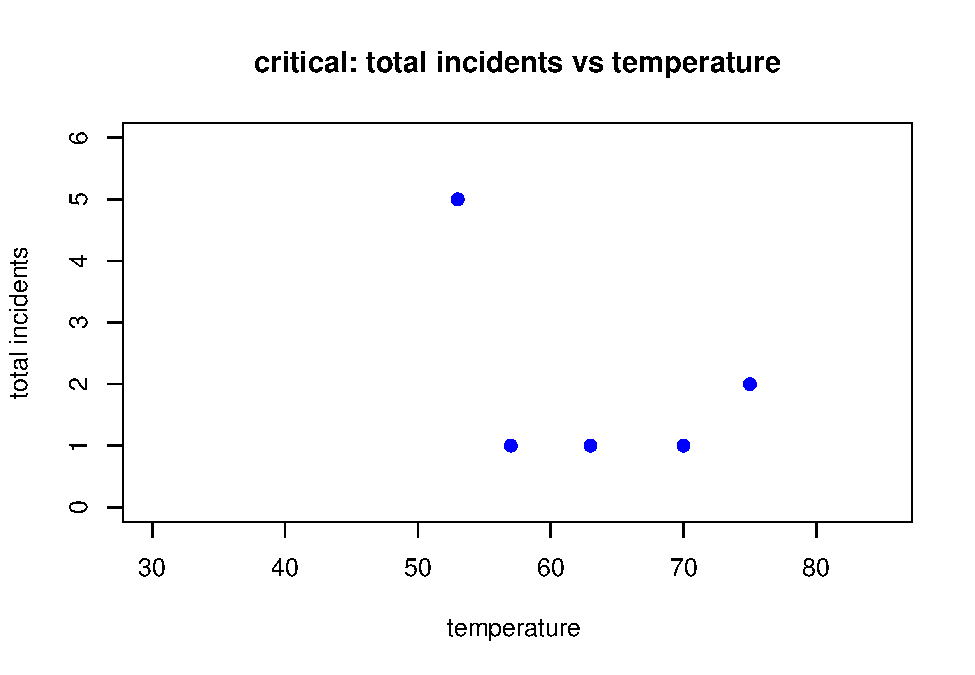
\includegraphics{3220103606-homework1_files/figure-latex/unnamed-chunk-12-1.pdf}

\begin{Shaded}
\begin{Highlighting}[]
\CommentTok{\# 绘制完整数据的图形}
\FunctionTok{plot}\NormalTok{(Total\_incidents }\SpecialCharTok{\textasciitilde{}}\NormalTok{ Temperature, }
     \AttributeTok{data =}\NormalTok{ orings,}
     \AttributeTok{main =} \StringTok{"full: total incidents vs temperature"}\NormalTok{,}
     \AttributeTok{xlab =} \StringTok{"temperature"}\NormalTok{, }
     \AttributeTok{ylab =} \StringTok{"total incidents"}\NormalTok{,}
     \AttributeTok{pch =} \DecValTok{19}\NormalTok{, }\AttributeTok{col =} \StringTok{"red"}\NormalTok{,}
     \AttributeTok{xlim =} \FunctionTok{c}\NormalTok{(}\DecValTok{30}\NormalTok{, }\DecValTok{85}\NormalTok{), }\AttributeTok{ylim =} \FunctionTok{c}\NormalTok{(}\DecValTok{0}\NormalTok{, }\DecValTok{6}\NormalTok{))}
\end{Highlighting}
\end{Shaded}

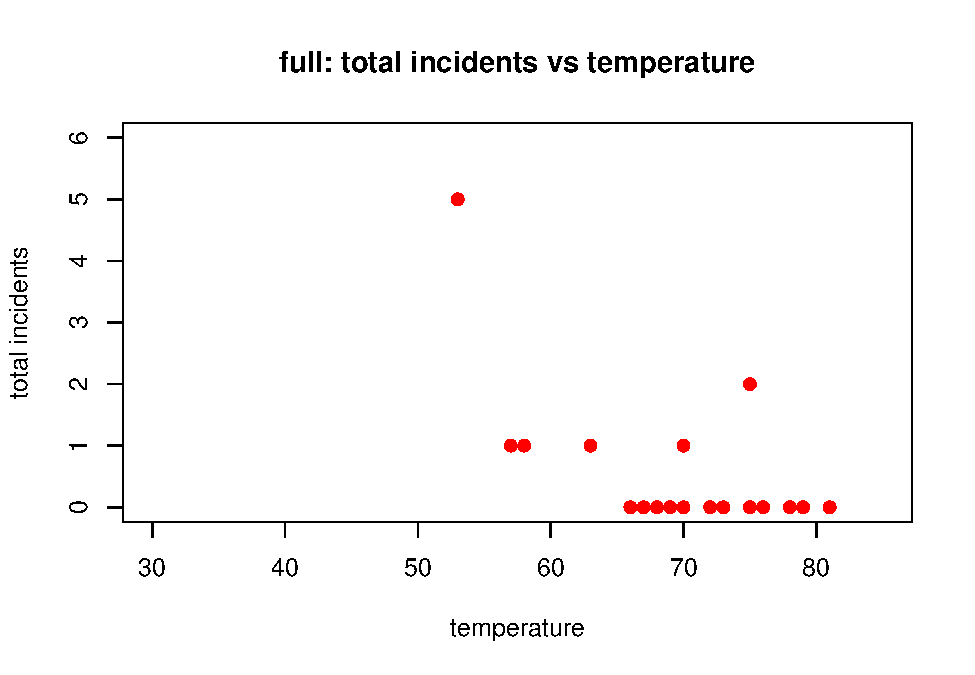
\includegraphics{3220103606-homework1_files/figure-latex/unnamed-chunk-12-2.pdf}

\subsection{MB.CH1.4}\label{mb.ch1.4}

\subsubsection{a.}\label{a.-3}

用以下代码解决问题。不存在缺失的列。

\begin{Shaded}
\begin{Highlighting}[]
\FunctionTok{library}\NormalTok{(DAAG)}

\FunctionTok{str}\NormalTok{(ais)}
\end{Highlighting}
\end{Shaded}

\begin{verbatim}
## 'data.frame':    202 obs. of  13 variables:
##  $ rcc   : num  3.96 4.41 4.14 4.11 4.45 4.1 4.31 4.42 4.3 4.51 ...
##  $ wcc   : num  7.5 8.3 5 5.3 6.8 4.4 5.3 5.7 8.9 4.4 ...
##  $ hc    : num  37.5 38.2 36.4 37.3 41.5 37.4 39.6 39.9 41.1 41.6 ...
##  $ hg    : num  12.3 12.7 11.6 12.6 14 12.5 12.8 13.2 13.5 12.7 ...
##  $ ferr  : num  60 68 21 69 29 42 73 44 41 44 ...
##  $ bmi   : num  20.6 20.7 21.9 21.9 19 ...
##  $ ssf   : num  109.1 102.8 104.6 126.4 80.3 ...
##  $ pcBfat: num  19.8 21.3 19.9 23.7 17.6 ...
##  $ lbm   : num  63.3 58.5 55.4 57.2 53.2 ...
##  $ ht    : num  196 190 178 185 185 ...
##  $ wt    : num  78.9 74.4 69.1 74.9 64.6 63.7 75.2 62.3 66.5 62.9 ...
##  $ sex   : Factor w/ 2 levels "f","m": 1 1 1 1 1 1 1 1 1 1 ...
##  $ sport : Factor w/ 10 levels "B_Ball","Field",..: 1 1 1 1 1 1 1 1 1 1 ...
\end{verbatim}

\begin{Shaded}
\begin{Highlighting}[]
\FunctionTok{colSums}\NormalTok{(}\FunctionTok{is.na}\NormalTok{(ais))}
\end{Highlighting}
\end{Shaded}

\begin{verbatim}
##    rcc    wcc     hc     hg   ferr    bmi    ssf pcBfat    lbm     ht     wt 
##      0      0      0      0      0      0      0      0      0      0      0 
##    sex  sport 
##      0      0
\end{verbatim}

\subsubsection{b.}\label{b.-3}

用一下代码解决问题。

\begin{Shaded}
\begin{Highlighting}[]
\CommentTok{\# 创建性别{-}运动项目交叉表}
\NormalTok{gender\_sport\_table }\OtherTok{\textless{}{-}} \FunctionTok{table}\NormalTok{(ais}\SpecialCharTok{$}\NormalTok{sport, ais}\SpecialCharTok{$}\NormalTok{sex)}

\CommentTok{\# 计算男女比例(男性比例)}
\NormalTok{male\_ratio }\OtherTok{\textless{}{-}}\NormalTok{ gender\_sport\_table[, }\StringTok{"m"}\NormalTok{] }\SpecialCharTok{/} \FunctionTok{rowSums}\NormalTok{(gender\_sport\_table)}

\CommentTok{\# 识别失衡项目(男性比例 \textgreater{} 2/3 或 \textless{} 1/3)}
\NormalTok{imbalanced\_sports }\OtherTok{\textless{}{-}} \FunctionTok{names}\NormalTok{(}\FunctionTok{which}\NormalTok{(male\_ratio }\SpecialCharTok{\textgreater{}} \DecValTok{2}\SpecialCharTok{/}\DecValTok{3} \SpecialCharTok{|}\NormalTok{ male\_ratio }\SpecialCharTok{\textless{}} \DecValTok{1}\SpecialCharTok{/}\DecValTok{3}\NormalTok{))}

\CommentTok{\# 打印结果}
\FunctionTok{print}\NormalTok{(}\StringTok{"性别{-}运动项目分布表:"}\NormalTok{)}
\end{Highlighting}
\end{Shaded}

\begin{verbatim}
## [1] "性别-运动项目分布表:"
\end{verbatim}

\begin{Shaded}
\begin{Highlighting}[]
\FunctionTok{print}\NormalTok{(gender\_sport\_table)}
\end{Highlighting}
\end{Shaded}

\begin{verbatim}
##          
##            f  m
##   B_Ball  13 12
##   Field    7 12
##   Gym      4  0
##   Netball 23  0
##   Row     22 15
##   Swim     9 13
##   T_400m  11 18
##   T_Sprnt  4 11
##   Tennis   7  4
##   W_Polo   0 17
\end{verbatim}

\begin{Shaded}
\begin{Highlighting}[]
\FunctionTok{cat}\NormalTok{(}\StringTok{"}\SpecialCharTok{\textbackslash{}n}\StringTok{性别比例失衡的运动项目(比例 \textgreater{} 2:1):"}\NormalTok{)}
\end{Highlighting}
\end{Shaded}

\begin{verbatim}
## 
## 性别比例失衡的运动项目(比例 > 2:1):
\end{verbatim}

\begin{Shaded}
\begin{Highlighting}[]
\FunctionTok{print}\NormalTok{(imbalanced\_sports)}
\end{Highlighting}
\end{Shaded}

\begin{verbatim}
## [1] "Gym"     "Netball" "T_Sprnt" "W_Polo"
\end{verbatim}

\subsection{MB.CH1.6}\label{mb.ch1.6}

\subsubsection{a.}\label{a.-4}

Y轴刻度:表示 log₂(面积)

Y轴增加1单位 → 面积翻倍 (2¹ = 2倍)

Y轴增加2单位 → 面积变为4倍 (2² = 4倍)

Y轴增加3单位 → 面积变为8倍 (2³ = 8倍)

点标签:

左侧数字:实际面积(km²)

右侧文字:湖泊名称

关键观察:

Winnipeg湖面积最大(log₂(24387) ≈ 14.6),远大于其他湖泊

Gods湖海拔最低但面积中等(178m, 1151km²)

海拔与面积无明显相关性

\begin{Shaded}
\begin{Highlighting}[]
\NormalTok{Manitoba.lakes }\OtherTok{\textless{}{-}} \FunctionTok{data.frame}\NormalTok{(}
  \AttributeTok{elevation =} \FunctionTok{c}\NormalTok{(}\DecValTok{217}\NormalTok{, }\DecValTok{254}\NormalTok{, }\DecValTok{248}\NormalTok{, }\DecValTok{254}\NormalTok{, }\DecValTok{253}\NormalTok{, }\DecValTok{227}\NormalTok{, }\DecValTok{178}\NormalTok{, }\DecValTok{207}\NormalTok{, }\DecValTok{217}\NormalTok{),}
  \AttributeTok{area =} \FunctionTok{c}\NormalTok{(}\DecValTok{24387}\NormalTok{, }\DecValTok{5374}\NormalTok{, }\DecValTok{4624}\NormalTok{, }\DecValTok{2247}\NormalTok{, }\DecValTok{1353}\NormalTok{, }\DecValTok{1223}\NormalTok{, }\DecValTok{1151}\NormalTok{, }\DecValTok{755}\NormalTok{, }\DecValTok{657}\NormalTok{)}
\NormalTok{)}

\FunctionTok{row.names}\NormalTok{(Manitoba.lakes) }\OtherTok{\textless{}{-}} \FunctionTok{c}\NormalTok{(}\StringTok{"Winnipeg"}\NormalTok{, }\StringTok{"Winnipegosis"}\NormalTok{, }\StringTok{"Manitoba"}\NormalTok{, }
                               \StringTok{"SouthernIndian"}\NormalTok{, }\StringTok{"Cedar"}\NormalTok{, }\StringTok{"Island"}\NormalTok{, }
                               \StringTok{"Gods"}\NormalTok{, }\StringTok{"Cross"}\NormalTok{, }\StringTok{"Playgreen"}\NormalTok{)}
\FunctionTok{attach}\NormalTok{(Manitoba.lakes)}

\FunctionTok{plot}\NormalTok{(elevation, }\FunctionTok{log2}\NormalTok{(area), }\AttributeTok{pch =} \DecValTok{16}\NormalTok{, }\AttributeTok{xlim =} \FunctionTok{c}\NormalTok{(}\DecValTok{170}\NormalTok{, }\DecValTok{280}\NormalTok{),}
     \AttributeTok{xlab =} \StringTok{"Elevation (m)"}\NormalTok{, }\AttributeTok{ylab =} \FunctionTok{expression}\NormalTok{(log[}\DecValTok{2}\NormalTok{](Area)),}
     \AttributeTok{main =} \StringTok{"Manitoba\textquotesingle{}s Largest Lakes (Logarithmic Scale)"}\NormalTok{)}

\FunctionTok{text}\NormalTok{(elevation, }\FunctionTok{log2}\NormalTok{(area), }\AttributeTok{labels =} \FunctionTok{row.names}\NormalTok{(Manitoba.lakes), }\AttributeTok{pos =} \DecValTok{4}\NormalTok{)}


\FunctionTok{text}\NormalTok{(elevation, }\FunctionTok{log2}\NormalTok{(area), }\AttributeTok{labels =}\NormalTok{ area, }\AttributeTok{pos =} \DecValTok{2}\NormalTok{)}

\FunctionTok{legend}\NormalTok{(}\StringTok{"topright"}\NormalTok{, }
       \AttributeTok{legend =} \FunctionTok{c}\NormalTok{(}\StringTok{"Left: Area (km*km)"}\NormalTok{, }\StringTok{"Right: Lake Name"}\NormalTok{),}
       \AttributeTok{text.col =} \FunctionTok{c}\NormalTok{(}\StringTok{"black"}\NormalTok{, }\StringTok{"black"}\NormalTok{), }\AttributeTok{bty =} \StringTok{"n"}\NormalTok{)}

\FunctionTok{mtext}\NormalTok{(}\StringTok{"Note: Each unit increase on y{-}axis represents doubling of lake area"}\NormalTok{, }
      \AttributeTok{side =} \DecValTok{1}\NormalTok{, }\AttributeTok{line =} \DecValTok{3}\NormalTok{, }\AttributeTok{cex =} \FloatTok{0.8}\NormalTok{)}
\end{Highlighting}
\end{Shaded}

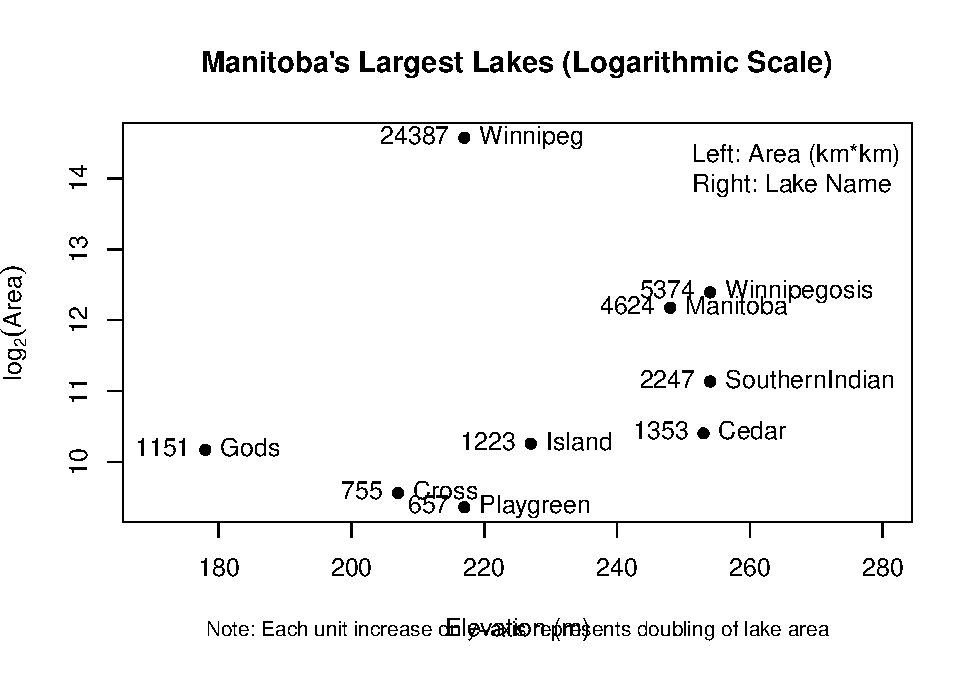
\includegraphics{3220103606-homework1_files/figure-latex/unnamed-chunk-15-1.pdf}

\subsubsection{b.}\label{b.-4}

Y轴刻度:对数变换后等距

从500到1000的距离 = 从1000到2000的距离(均表示面积翻倍)

大湖(Winnipeg)与小湖(Cross)差异更明显

优势:

直接显示实际面积值

保持面积比例关系直观

避免Winnipeg湖压缩其他数据点

与(a)对比:

相同的数据关系

不同的视觉表示

对数Y轴图更易解释面积差异

\begin{Shaded}
\begin{Highlighting}[]
\CommentTok{\# 创建对数Y轴图形}
\FunctionTok{plot}\NormalTok{(area }\SpecialCharTok{\textasciitilde{}}\NormalTok{ elevation, }\AttributeTok{data =}\NormalTok{ Manitoba.lakes, }\AttributeTok{pch =} \DecValTok{16}\NormalTok{, }
     \AttributeTok{xlim =} \FunctionTok{c}\NormalTok{(}\DecValTok{170}\NormalTok{, }\DecValTok{280}\NormalTok{), }\AttributeTok{log =} \StringTok{"y"}\NormalTok{,}
     \AttributeTok{xlab =} \StringTok{"Elevation (m)"}\NormalTok{, }\AttributeTok{ylab =} \StringTok{"Area (km*km)"}\NormalTok{,}
     \AttributeTok{main =} \StringTok{"Manitoba\textquotesingle{}s Largest Lakes (Logarithmic Y{-}axis)"}\NormalTok{,}
     \AttributeTok{yaxt =} \StringTok{"n"}\NormalTok{)  }\CommentTok{\# 禁用默认Y轴}

\CommentTok{\# 添加自定义对数刻度}
\FunctionTok{axis}\NormalTok{(}\DecValTok{2}\NormalTok{, }\AttributeTok{at =} \FunctionTok{c}\NormalTok{(}\DecValTok{500}\NormalTok{, }\DecValTok{1000}\NormalTok{, }\DecValTok{2000}\NormalTok{, }\DecValTok{5000}\NormalTok{, }\DecValTok{10000}\NormalTok{, }\DecValTok{20000}\NormalTok{), }
     \AttributeTok{labels =} \FunctionTok{c}\NormalTok{(}\StringTok{"500"}\NormalTok{, }\StringTok{"1,000"}\NormalTok{, }\StringTok{"2,000"}\NormalTok{, }\StringTok{"5,000"}\NormalTok{, }\StringTok{"10,000"}\NormalTok{, }\StringTok{"20,000"}\NormalTok{))}

\CommentTok{\# 添加湖泊名称标签 (右侧)}
\FunctionTok{text}\NormalTok{(Manitoba.lakes}\SpecialCharTok{$}\NormalTok{elevation, Manitoba.lakes}\SpecialCharTok{$}\NormalTok{area, }
     \AttributeTok{labels =} \FunctionTok{row.names}\NormalTok{(Manitoba.lakes), }\AttributeTok{pos =} \DecValTok{4}\NormalTok{)}

\CommentTok{\# 添加面积数值标签 (左侧)}
\FunctionTok{text}\NormalTok{(Manitoba.lakes}\SpecialCharTok{$}\NormalTok{elevation, Manitoba.lakes}\SpecialCharTok{$}\NormalTok{area, }
     \AttributeTok{labels =}\NormalTok{ Manitoba.lakes}\SpecialCharTok{$}\NormalTok{area, }\AttributeTok{pos =} \DecValTok{2}\NormalTok{)}

\CommentTok{\# 添加比例解释}
\FunctionTok{mtext}\NormalTok{(}\StringTok{"Note: Vertical distances represent multiplicative differences in area"}\NormalTok{, }
      \AttributeTok{side =} \DecValTok{1}\NormalTok{, }\AttributeTok{line =} \DecValTok{3}\NormalTok{, }\AttributeTok{cex =} \FloatTok{0.8}\NormalTok{)}
\end{Highlighting}
\end{Shaded}

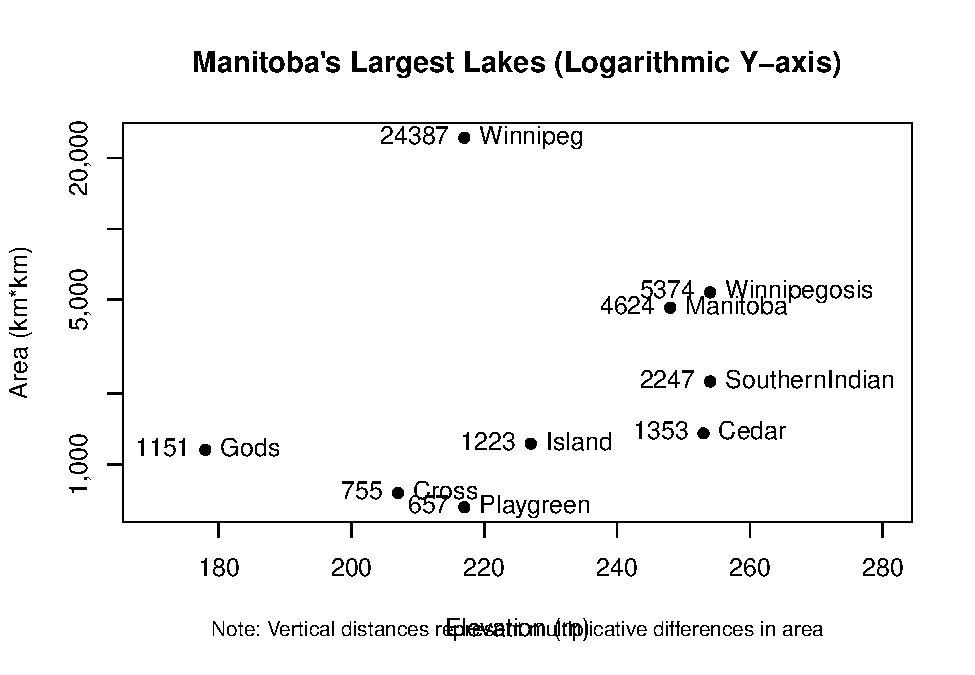
\includegraphics{3220103606-homework1_files/figure-latex/unnamed-chunk-16-1.pdf}

关键结论:两种对数表示都揭示了Winnipeg湖的绝对主导地位(占所有湖泊总面积的约70\%),但未显示海拔与面积的显著相关性。对数变换对于可视化跨度大的面积数据至关重要。

\subsection{MB.CH1.7}\label{mb.ch1.7}

用以下代码完成。

\begin{Shaded}
\begin{Highlighting}[]
\NormalTok{Manitoba.lakes }\OtherTok{\textless{}{-}} \FunctionTok{data.frame}\NormalTok{(}
  \AttributeTok{elevation =} \FunctionTok{c}\NormalTok{(}\DecValTok{217}\NormalTok{, }\DecValTok{254}\NormalTok{, }\DecValTok{248}\NormalTok{, }\DecValTok{254}\NormalTok{, }\DecValTok{253}\NormalTok{, }\DecValTok{227}\NormalTok{, }\DecValTok{178}\NormalTok{, }\DecValTok{207}\NormalTok{, }\DecValTok{217}\NormalTok{),}
  \AttributeTok{area =} \FunctionTok{c}\NormalTok{(}\DecValTok{24387}\NormalTok{, }\DecValTok{5374}\NormalTok{, }\DecValTok{4624}\NormalTok{, }\DecValTok{2247}\NormalTok{, }\DecValTok{1353}\NormalTok{, }\DecValTok{1223}\NormalTok{, }\DecValTok{1151}\NormalTok{, }\DecValTok{755}\NormalTok{, }\DecValTok{657}\NormalTok{)}
\NormalTok{)}

\FunctionTok{rownames}\NormalTok{(Manitoba.lakes) }\OtherTok{\textless{}{-}} \FunctionTok{c}\NormalTok{(}\StringTok{"Winnipeg"}\NormalTok{, }\StringTok{"Winnipegosis"}\NormalTok{, }\StringTok{"Manitoba"}\NormalTok{, }
                             \StringTok{"SouthernIndian"}\NormalTok{, }\StringTok{"Cedar"}\NormalTok{, }\StringTok{"Island"}\NormalTok{, }
                             \StringTok{"Gods"}\NormalTok{, }\StringTok{"Cross"}\NormalTok{, }\StringTok{"Playgreen"}\NormalTok{)}


\CommentTok{\# (a) linear scale}
\FunctionTok{dotchart}\NormalTok{(Manitoba.lakes}\SpecialCharTok{$}\NormalTok{area,}
         \AttributeTok{labels =} \FunctionTok{rownames}\NormalTok{(Manitoba.lakes),}
         \AttributeTok{main =} \StringTok{"lake Area (linear scale)"}\NormalTok{,}
         \AttributeTok{xlab =} \StringTok{"Area (km*km)"}\NormalTok{,}
         \AttributeTok{pch =} \DecValTok{19}\NormalTok{, }\AttributeTok{col =} \StringTok{"blue"}\NormalTok{,}
         \AttributeTok{cex =} \FloatTok{0.8}\NormalTok{)}
\end{Highlighting}
\end{Shaded}

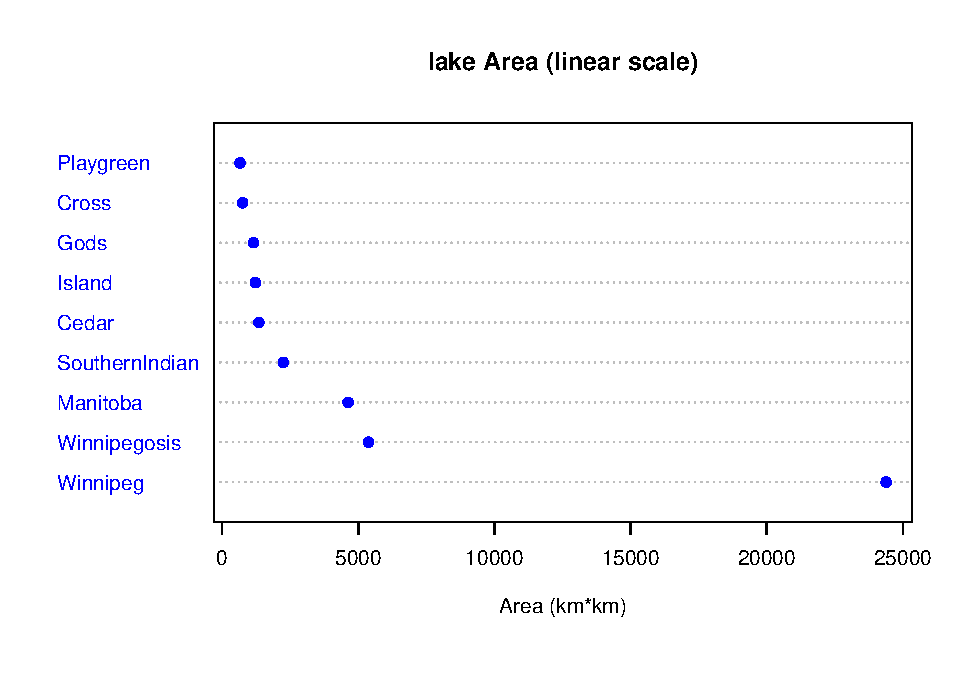
\includegraphics{3220103606-homework1_files/figure-latex/unnamed-chunk-17-1.pdf}

\begin{Shaded}
\begin{Highlighting}[]
\CommentTok{\# (b) logarithmic scale}
\FunctionTok{dotchart}\NormalTok{(}\FunctionTok{log2}\NormalTok{(Manitoba.lakes}\SpecialCharTok{$}\NormalTok{area),}
         \AttributeTok{labels =} \FunctionTok{rownames}\NormalTok{(Manitoba.lakes),}
         \AttributeTok{main =} \StringTok{"lake Area (logarithmic scale: log₂)"}\NormalTok{,}
         \AttributeTok{xlab =} \StringTok{"log2(Area)"}\NormalTok{,}
         \AttributeTok{pch =} \DecValTok{19}\NormalTok{, }\AttributeTok{col =} \StringTok{"red"}\NormalTok{,}
         \AttributeTok{cex =} \FloatTok{0.8}\NormalTok{)}
\end{Highlighting}
\end{Shaded}

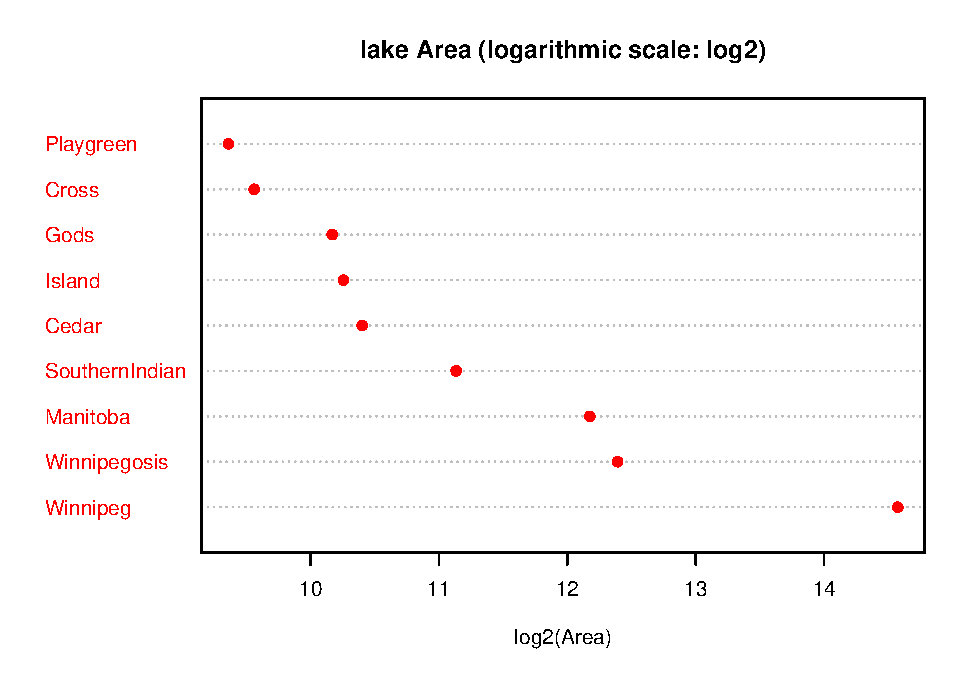
\includegraphics{3220103606-homework1_files/figure-latex/unnamed-chunk-17-2.pdf}

\subsection{MB.CH1.8}\label{mb.ch1.8}

\begin{Shaded}
\begin{Highlighting}[]
\NormalTok{Manitoba.lakes }\OtherTok{\textless{}{-}} \FunctionTok{data.frame}\NormalTok{(}
  \AttributeTok{elevation =} \FunctionTok{c}\NormalTok{(}\DecValTok{217}\NormalTok{, }\DecValTok{254}\NormalTok{, }\DecValTok{248}\NormalTok{, }\DecValTok{254}\NormalTok{, }\DecValTok{253}\NormalTok{, }\DecValTok{227}\NormalTok{, }\DecValTok{178}\NormalTok{, }\DecValTok{207}\NormalTok{, }\DecValTok{217}\NormalTok{),}
  \AttributeTok{area =} \FunctionTok{c}\NormalTok{(}\DecValTok{24387}\NormalTok{, }\DecValTok{5374}\NormalTok{, }\DecValTok{4624}\NormalTok{, }\DecValTok{2247}\NormalTok{, }\DecValTok{1353}\NormalTok{, }\DecValTok{1223}\NormalTok{, }\DecValTok{1151}\NormalTok{, }\DecValTok{755}\NormalTok{, }\DecValTok{657}\NormalTok{),}
  \AttributeTok{row.names =} \FunctionTok{c}\NormalTok{(}\StringTok{"Winnipeg"}\NormalTok{, }\StringTok{"Winnipegosis"}\NormalTok{, }\StringTok{"Manitoba"}\NormalTok{, }\StringTok{"SouthernIndian"}\NormalTok{, }
                \StringTok{"Cedar"}\NormalTok{, }\StringTok{"Island"}\NormalTok{, }\StringTok{"Gods"}\NormalTok{, }\StringTok{"Cross"}\NormalTok{, }\StringTok{"Playgreen"}\NormalTok{)}
\NormalTok{)}

\CommentTok{\# 计算水域面积下界}
\NormalTok{water\_area\_lower\_bound }\OtherTok{\textless{}{-}} \FunctionTok{sum}\NormalTok{(Manitoba.lakes}\SpecialCharTok{$}\NormalTok{area)}

\CommentTok{\# 显示结果}
\FunctionTok{cat}\NormalTok{(}\StringTok{"马尼托巴省水域面积下界:"}\NormalTok{, }
    \FunctionTok{format}\NormalTok{(water\_area\_lower\_bound, }\AttributeTok{big.mark =} \StringTok{","}\NormalTok{), }
    \StringTok{"平方公里}\SpecialCharTok{\textbackslash{}n}\StringTok{"}\NormalTok{)}
\end{Highlighting}
\end{Shaded}

\begin{verbatim}
## 马尼托巴省水域面积下界: 41,771 平方公里
\end{verbatim}

\begin{Shaded}
\begin{Highlighting}[]
\FunctionTok{cat}\NormalTok{(}\StringTok{"}\SpecialCharTok{\textbackslash{}n}\StringTok{说明:"}\NormalTok{,}
    \StringTok{"}\SpecialCharTok{\textbackslash{}n}\StringTok{• 此计算基于马尼托巴省9个主要湖泊的面积总和"}\NormalTok{,}
    \StringTok{"}\SpecialCharTok{\textbackslash{}n}\StringTok{• 实际水域面积更大(包含未统计的小型湖泊、河流和湿地)"}\NormalTok{,}
    \StringTok{"}\SpecialCharTok{\textbackslash{}n}\StringTok{• 因此"}\NormalTok{, }\FunctionTok{format}\NormalTok{(water\_area\_lower\_bound, }\AttributeTok{big.mark =} \StringTok{","}\NormalTok{), }
    \StringTok{"平方公里仅为最小估计值"}\NormalTok{)}
\end{Highlighting}
\end{Shaded}

\begin{verbatim}
## 
## 说明: 
## • 此计算基于马尼托巴省9个主要湖泊的面积总和 
## • 实际水域面积更大(包含未统计的小型湖泊、河流和湿地) 
## • 因此 41,771 平方公里仅为最小估计值
\end{verbatim}

\end{document}
